\chapter{OpenNES}
\thispagestyle{standard}
\pagestyle{standard}
\renewcommand{\footrulewidth}{0.4pt}
\lfoot{\small Refik Kerimi}

Wie in Kapitel \ref{chap:Einleitung} beschrieben, hat der stetige Zuwachs von \acs{DER}-Systemen zum Umdenken bei der Planung und beim Betreiben von Stromnetzen geführt \cite{DERs}.
Das Konzept der \ac {SGSY} ermöglicht die Verwendung von existierenden Anlagen auf eine effizientere Art und Weise und trägt damit zu einem höheren Marktanteil von DER Systemen bei.
Solche Ansätze erfordern neue Lösungen in der \acl{IKT}, Automatisierungsarchitektur und in der Steuerung der Systeme.  
OpenNES umfasst das Konzept, wie in  \upshape \cite{Fronius} beschrieben und in Abbildung \ref{fig:Übersicht des OpenNES Konzepts} dargestellt, einer \acs{IKT}-Lösung zur Integration von erneuerbaren Energiequellen in  \acs {SGSY}  \cite{SmartGrids}. Die Entwicklung beschäftigt sich mit fernprogrammierbaren Funktionen, generischen Kommunikationsstrukturen sowie dazugehörigen Anwendungsmodellierungsmethoden für \acs{DER} Komponenten.
Einen weiteren Schwerpunkt von OpenNES stellt der Zugriff auf die \acs{DER} Systeme dar, wobei die unterschiedlichen Benutzerrollen berücksichtigt werden müssen.
OpenNES nimmt im Bereich der \acs{SGSY} eine zentrale Rolle ein, da es eine Open Source Plattform bietet. 



\begin{figure}[h]
	\centering
	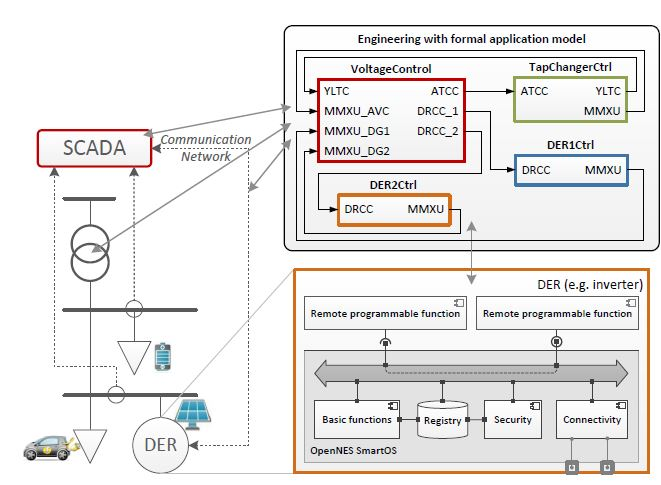
\includegraphics[width=14cm]{BilderAllgemein/OpenNES_architecture}\medskip
	\caption{Übersicht des OpenNES Konzepts \cite{OpenNES}}
	\label{fig:Übersicht des OpenNES Konzepts}
\end{figure}

 
\section{OpenNES SmartOS}
Das OpenNES Smart OS ist die Softwareplattform von OpenNES \upshape \cite{Fronius}. 
Es ist eine Plattform zur Steuerung von \acs{DER} Komponenten, mit dem Ziel die Flexibilität, die Erweiterungsmöglichkeiten und die Kompatibilität zu erhöhen.
In Abbildung \ref{fig:OpenNES System Architektur} ist das SmartOS von OpenNES zu sehen. Die Steuerungsplattform beinhaltet drei Hauptkomponenten:
\begin{itemize}
    \item Das Betriebssystem mit den Basis- und Kommunikationsfunktionen
	\item Das Sicherheitsmodul und austauschbare \ac{SWK}
	\item Die Entwicklungsumgebung um die \acs{SWK} zu programmieren oder neu zu konfigurieren
\end{itemize}

Das SmartOS ist kein normales Betriebssystem, sondern es besteht aus verschiedenen Abstraktionsschichten mit zusätzlicher Funktionalität zum Behandeln der Softwarekomponenten und dessen Interaktionen.


\begin{figure}[h]
	\centering
	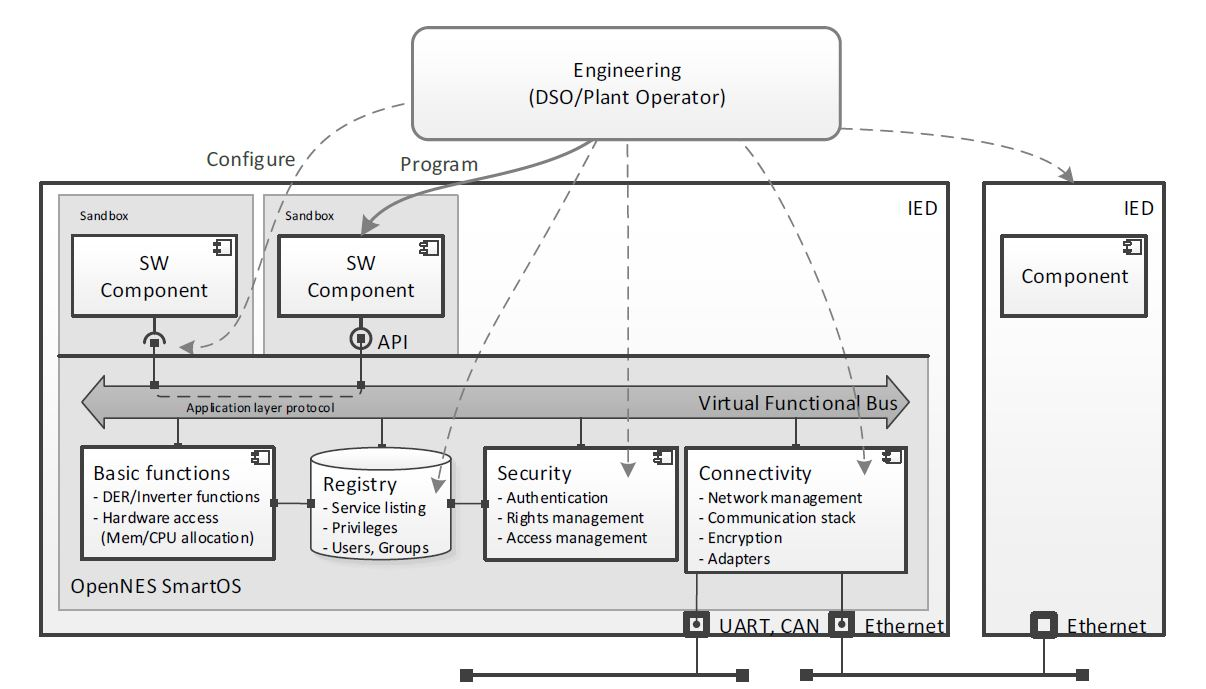
\includegraphics[width=14cm]{BilderAllgemein/ON_Smart_OS}\medskip
	\caption{OpenNES System Architektur \cite{OpenNES}}
	\label{fig:OpenNES System Architektur}
\end{figure}


\newpage
\section{Basisfunktionen}
Wie in Abbildung \ref{fig:Übersicht des OpenNES Konzepts} zu sehen ist, beinhaltet das Basis Funktionsmodul Standardmethoden für \acs{DER}/Inverter Systeme \cite{OpenNES}. Dieses interne Modul bietet Funktionen zur Unterstützung der Stromnetzwerke.
Aktuell dienen die Funktionen in erster Linie dazu, die Einspeiseleistung zu maximieren, indem die negativen Auswirkungen auf die Netzparameter (Spannung, Frequenz) möglichst minimiert werden und verhindert wird, dass das Netz destabilisiert wird.
OpenNES bietet Netzbetreibern eine gezielte, aktive Unterstützung, um Systeme und den Stromfluss großflächig zu beeinflussen. 
Es können weitere DERs (z.B.: Photovoltaik Anlagen) ohne den Ausbau der Netze (engl. Grid Enforcement) installiert werden.
Diese Funktionen und Verhaltensmuster werden mit der Bezeichnung \ac{AGF} gekennzeichnet und dienen dazu, Anforderungen an das System zu bewältigen.

\section{Softwarekomponenten}
Die \ac{SWK} sind als eigenständiger Bestandteil in das SmartOS eingebunden. Sie sind austauschbar, dass heißt man kann die Komponenten dynamisch hinzufügen oder entfernen, ohne dass man das System neu kompilieren muss.
Diese können entweder von den DER Herstellern oder von einem zertifizierten externen Anbieter entwickelt und geliefert werden und in verschiedenen Sprachen bzw. mit Hilfe verschiedener Technologien implementiert werden.\\
Wichtig für die Sicherheit ist, dass die \acs{SWK} in einer sicheren Umgebung eingekapselt werden wie in Abbildung \ref{fig:Softwarekomponente} zu sehen ist. Dies wird durch die Sandbox Methode erreicht, d.h dass sie von den Systemressourcen isoliert werden. Sie werden in einer Laufzeitumgebung z.B.: Java Runtime Environment ausgeführt. Dies ermöglicht eine weitere Verkapselung aus dem System.
Dadurch haben die \acs{SWK} einen eingeschränkten Zugang z.B. auf Speicher- und Dateiverwaltung. Jede Komponente kann über den \ac{VFB} Dienste angeben, bereitstellen und anfordern. Das Updaten und Programmieren der Komponenten kann während der Laufzeit erfolgen. Dies bringt einige Vorteile wie z.B.: neue Funktionalitäten oder das Rekonfigurieren der Komponenten, aber auch Gefahren mit sich.
Es sollte sichergestellt werden, dass die Anwendung nur innerhalb bestimmter Einschränkungen arbeitet, z.B.: das Ändern der Blindleistung der \acs{DER} nur zwischen +/- 10\% der Nennleistung.


\begin{figure}[H]
	\centering
	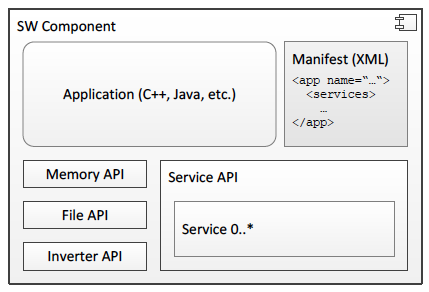
\includegraphics[width=8cm]{BilderAllgemein/SWK}\medskip
	\caption{Softwarekomponente \cite{Fronius}}
	\label{fig:Softwarekomponente}
\end{figure}

\section{Sicherheitsmodul}
Jegliche Art von Kommunikation zwischen den Komponenten, auch jene zwischen den Softwarekomponenten des gleichen Geräts, müssen durch das Sicherheitsmodul autorisiert werden. Die Sicherheit wird über die rollenbasierte Zugriffskontrolle (RBAC) geregelt und dient als Zugriffspunkt. Für jede Zugriffsanforderung werden die Zugriffsrechte durch das Modul bestimmt. Der \acs{VFB} verarbeitet nur die Daten, die vom Sicherheitsmodul genehmigt wurden \cite{OpenNES, securityByDesign}.

\section{Virtual Functional Bus}
Der \acs{VFB} ermöglicht die Kommunikation zwischen den einzelnen Komponenten. Alle Software Komponenten können über eine API Schnittelle Dienste anbieten oder beziehen.
Die API wird vom OpenNES Smart OS über den VFB zur Verfügung gestellt.
Die Dienste sind rein intern oder extern zugänglich \cite{OpenNES}. 

\section{Registrierung}
Das Registrierungsmodul beinhaltet alle Benutzer oder Gruppen, die dem \ac{IED} bekannt sind, sowie die Berechtigungen und die Daten der Software Komponenten \cite{OpenNES}. Dieses Modul ist der Berechtigungsspeicher des OpenNES Systems. 

\newpage
\section{Connectivity Modul} \label{CM}

\begin{figure}[h]
	\centering
	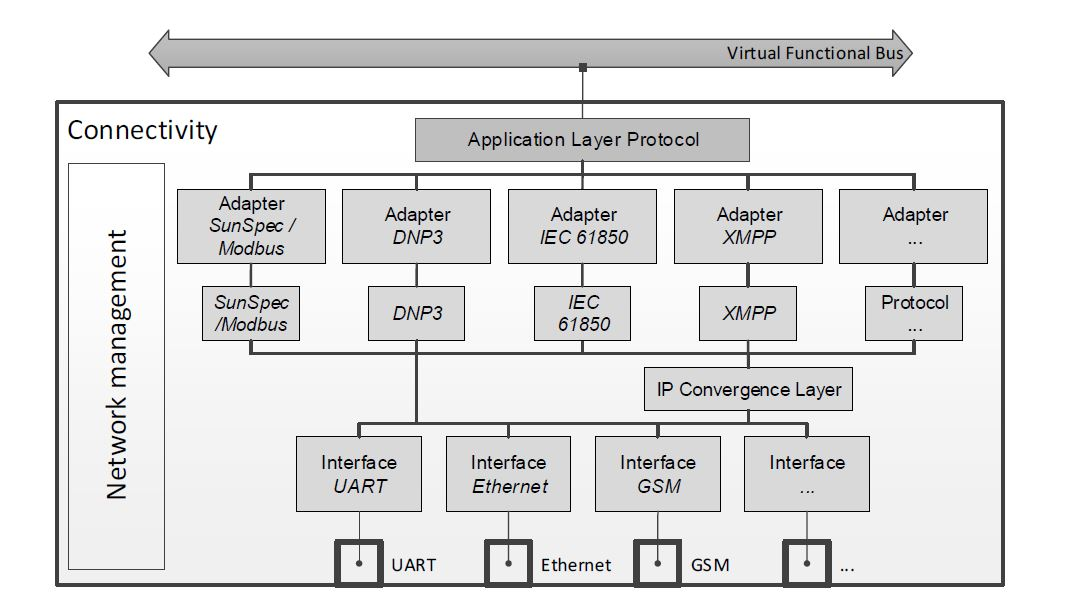
\includegraphics[width=14cm]{BilderAllgemein/CN_Module}\medskip
	\caption{Connectivity Modul \cite{OpenNES}}
	\label{fig:OpenNESConnectivityModule}
\end{figure}

Das \ac{CM} (Abbildung \ref{fig:OpenNESConnectivityModule}) beinhaltet die Schnittstellen zur externen Kommunikation über den virtuellen Bus welcher als \ac{VFB}  bezeichnet wird \cite{OpenNES}. Diese Projektarbeit konzentriert sich hauptsächlich, auf dieses Modul.
Durch die Verwendung von Protokolladaptern werden die Flexibilität und die Erweiterungsmöglichkeiten des Systems erhöht.
Protokolladapter werden verwendet, um zwischen den verschiedenen Verbindungsmethoden und den einheitlichen Protokollen der Anwendungsschicht zu übersetzten.
Auch werden die Adapter dazu verwendet, fehlende Funktionen und Kommunikationsschema wie z.B.: publish-subscribe, request-response, push massaging pattern u.a. anbieten zu können.




















